\documentclass[fsharpNotes.tex]{subfiles}
\graphicspath{ {./figures/} }

\begin{document}
\chapter{Data Structures}
\label{chap:dataStructures}

\abstract{
  A data structure is an organization of collections of data, such that operations on them are efficient. In earlier chapters, we have already looked at some examples, e.g.,
  \begin{itemize}
  \item strings which are variable length sequences of characters and which were discussed in \Cref{chap:calculator},
  \item tuples which are fixed length sequences of values of variable types and which were discussed in \Cref{sec:tuples},
  \item lists which are variable length sequences of values of identical type and which were discussed in \Cref{chap:lists}, and
  \item stacks which are specialized lists, where values can only be added and removed from its head, and which was discussed in \Cref{sec:stack}.
  \end{itemize}
In this chapter, we will further consider the following data structures:
  \begin{itemize}
  \item \idx{queues} which are specialized lists, where elements can be added to the end of the list and removed from its head,
  \item \idx{trees} which are hierarchical orderings of data of a variable number of values of identical types,
%  \item \idx{graphs} which are networks of nodes,
  \item \idx{sets} which are an unordered collection of unique values of the identical type, and
  \item \idx{hash maps} which are mappings between sets of keys into sets of values. 
  \end{itemize}
  These data structures have a long history and are often discussed from an abstract point of view in terms of their conceptual interface and from a computational complexity point of view, where details of their implementation are stressed. The above-mentioned data structures occur frequently alone or in combination with many programming solutions and form a solid basis for solving problems by programming. Some of these data structures have their predefined modules in F\# but not all. In this chapter, we will give a brief introduction to each.}


\section{Queues}
A queue is a sequence values that can be added to its end and removed from its front as illustrated in \Cref{fig:queue}.
\begin{figure}
  \centering
  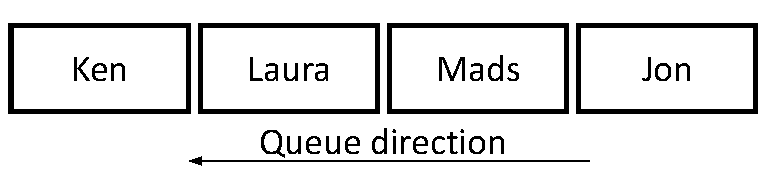
\includegraphics[width=0.6\linewidth]{queue}
  \caption{A queue with Ken in the front and Jon in the back of the queue.}
  \label{fig:queue}
\end{figure}
Queues appear often in real life: Standing in line at a shop counter, orders await in a queue for their turn to be shipped in an online shop, and students waiting to be examined at an oral examination. Many operations on queues can be defined, but the following are always present in some form:
\begin{description}
\item[create:] Create an empty queue.
\item[enqueue:] Add an element to the back of the queue.
\item[dequeue:] Remove the element at the front of the queue.
\item[head:] Get the value of the front element of the queue.
\item[isEmpty:] Check if the queue is empty.
\end{description}
As of the writing of this book, the standard collection of Fsharp libraries does not include a queues module, but they can easily be implemented using lists. For example, a queue of integers is implemented in \Cref{queueImplementation}.
%
\fsImplementation{queue}{queueImplementation}{Implementing a functional queue using lists.}{}
%
This is a functional queue because the enqueue and dequeue operations return a new queue they are called, without destroying the old queue. Mutable queues are more common, where en- and dequeuing update the value of a queue as a side-effect. See \Cref{sec:mutableValues} for more on mutable values. A simple application using this queue is shown in \Cref{queueApp}
%
\fs{queueApp}{An application of the Queue module.}
%
Note that this implementation, the computational complexity of all but \lstinline{enqueue} is $\mathcal{O}(1)$, while \lstinline{enqueue} is $\mathcal{O}(n)$, where $n$ is the length of the list, since it relies on list concatenation. Faster implementations exist but are beyond the scope of this book.

\section{Trees}
A tree is a hierarchical organization of data. For example the expression
\begin{equation}
\frac{1}{3+5}
\end{equation}
can be represented as shown in \Cref{fig:tree}
\begin{figure}
  \centering
  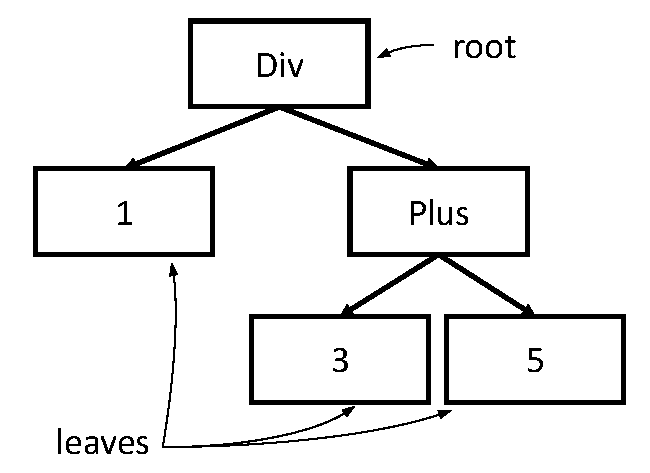
\includegraphics[width=0.45\linewidth]{tree}
  \caption{A tree representation of $1/(3+5)$.}
  \label{fig:tree}
\end{figure}
Further examples of trees are the file structure on your hard disk, where a directory contains files and other directories, and the list of contents of this book, which has chapters consisting of sections which in turn consist of subsections.

Trees consists of \idx[node]{nodes} and \idx[relation]{relations}. In \Cref{fig:tree}, 1, 3, 5, ``Div'', and ``Plus'' are nodes and their relation are shown with arrows. Relations are often described as family relations, such that, e.g., 1 and ``Plus'' are \idx{siblings} and are the \idx[child]{children} of the \idx{parent} ``Div''. Nodes which do not have \idx[descendant]{descendants} are called \idx[leaf]{leaves}, and there must be on node, which does not have \idx[ancestor]{ancestors} and that is called the \idx{root}. Trees are often classified as being \idx{$k$-ary}, if each node has at most  $k$ children. The example in \Cref{fig:tree} is an example of a 2-ary or \idx{binary tree}. Trees are often displayed with the children below their parent, in which case the arrowheads are neglected. 


As of the writing of this book, the standard collection of Fsharp libraries does not include a tree module. Trees are somewhat complicated to program in the functional paradigm since they are non-linear structures. One way to represent them is with the use of discriminated union, as demonstrated in \Cref{bTreeCode}.
%
\fsCode{bTree}{bTreeCode}{Representing a computational expression as a binary tree}{}
% 
Such values are not easy to read, since it relies on nested types and tuples. Luckily, it is not difficult to make a function, which converts the tree into a string for later displaying on the screen. Such functions are commonly called \idx[toString@\lstinline{toString}]{\lstinline{toString}} and will be discussed later in \Cref{oop}. Here, the strategy will be to increase indentation proportional to the depth of the nodes printed, and one version of \lstinline{toString} is shown in \Cref{bTreeToString}
%
\fs{bTreeToString}{A \lstinline!toString!  method aids the interpretation of tree values.}
%
The result is to be interpreted as \lstinline{Div} is the division operation of a \lstinline{Value 1.0) and the result of performing the \lstinline{Plus} of two other values.
  
  The \lstinline{toString} function is an example of tree traversal. For binary trees 3 different traversal orders are common: \idx[prefix traversal]{Prefix}, \idx[infix traversal]{infix} and \idx[postfix traversal]{postfix} order according to the order in which the value of a node and its two children are handled. Consider a node with a value \lstinline{elm} and its two children \lstinline{left} and \lstinline{right}, the ordering is as follows:
\begin{description}
\item[Prefix order:] \lstinline{elm}, \lstinline{left}, and \lstinline{right}
\item[Infix order:] \lstinline{left}, \lstinline{elm}, and \lstinline{right}
\item[Postfix order:] \lstinline{left}, \lstinline{right}, and \lstinline{elm} 
\end{description}
Thus, \lstinline{toString} in \Cref{bTreeToString} is a prefix traversal. In \Cref{bTreeTraversal} the 3 traversal schemes are used to convert a binary tree to a list of \lstinline{element} values.
%
\fs{bTreeTraversal}{Pre-, in-, and postfix traversal of a binary tree.}
%

Traversal methods linearize the tree structure and in general, 2 different traversals are required to reconstruct the original tree. However, as we saw in \Cref{sec:stack}, a stack can be used to properly evaluate postfix representations of mathematical expressions. The code in \Cref{postfixAppGeneric} can be modified for this purpose. Firstly, no computations need to be done, but every operator must result in a node and every value in a leaf, and instead of a stack of values, we must stack the sub-trees. The result is shown in \Cref{bTreeFromPostfix}.
% 
\fs{bTreeFromPostfix}{Using a stack to reconstruct a tree from its postfix traversal.}
%
Note that the resulting element on the stack is the original tree as expected.

\section{Programming intermezzo: Sorting Integers with a Binary Tree}
Consider the problem of sorting a list of integers
\begin{task}{probl:sortingBTree}
  Given a list of integers, such as \lstinline{[5; 5; 7; 8; 3; 1; 8; 9; 0; 8]}, sort them and print the result on the screen.
\end{task}
This is such a common task that the list module contains a function for just this, \lstinline{List.sort}, but here we will use the problem to study programming with binary trees. Our strategy will be to build a generic library for binary trees and an application with a function for sorting these values.

A strategy for sorting values is to enter them into a binary tree such that a node's value is always larger than its left child and less than or equal to its right child. The list could thus result in the tree shown in \Cref{fig:sortedBTree}.
\begin{figure}
  \begin{center}
    \begin{tikzpicture}
      [
      level 1/.style = {sibling distance = 4cm},
      level 2/.style = {sibling distance = 2.5cm}
      ]
      
      \node {5}
      child {node {1}
        child [missing] {[fill] circle (2pt)}
        child {node {3}}
        edge from parent} 
      child {node {8}
        child {node {5}}
        child {node {9}}
        edge from parent};
    \end{tikzpicture}
  \end{center}
  \caption{A binary sorting tree for the list \lstinline{[5; 1; 8; 3; 9; 5]}.}
  \label{fig:sortedBTree}
\end{figure}
A consequence of the sorting rule is that given a node, then its value is larger than all the values in the left sub-tree and no bigger than any values in the right sub-tree. Note also that the infix traversal of the tree gives a sorted list of values. In \Cref{fig:sortedBTree} this is \lstinline{[1; 3; 5; 5; 8; 9]}. In the spirit of our 8-step guide, let us make a sketch of the sorting algorithm to get a feeling of which types and functions could be useful. Firstly, we will need a generator of random numbers, to make sure we test many different combinations. This can be achieved with \lstinline{System.Random()} and \lstinline{List.map} as shown in \Cref{sortGenerator}
%
\fsCode{bTreeSort}{sortGenerator}{Generating a list of random integers in the interval 0 to 9.}{firstnumber=16,firstline=16,lastline=17} % Absolute reference!
%
Then we will need a type for a tree, and here we will use a generic type \lstinline{bTree<'a>}, such that we reuse it for other values that can be compared with the $\le$ operator. Our idea is to take the elements in the unsorted list to be inserted into a tree sequentially, and then finally write the result using infix traversal, e.g., as shown in \Cref{sortFold}
%
\fsCode{bTreeSort}{sortFold}{Using \lstinline{List.fold} to sequentially insert integers into a binary sorting tree.}{firstnumber=18,firstline=18,lastline=19} % Absolute reference!
%
Working with this, we realize that we will need a method for creating tree nodes and inserting them in a sorted fashion into a tree. Hence, we suggest the functions
\begin{quote}
  \lstinline{create: v: 'a -> bTree<'a>}\\
  \lstinline{sortInsert: acc: bTree<'a> -> elm: 'a -> bTree<'a>}
\end{quote}
Given a value, the function \lstinline{sortInsert} must start at the root of the tree and traverse down the tree until it finds a node with space for a leaf that obeys the sorting rule. Thinking about this, we realize, that the tree type could well make use of the option type, e.g.,
\begin{quote}
  \lstinline{type bTree<'a> = Node of 'a * bTree<'a> option * bTree<'a> option}\\
\end{quote}
and thus, an available position can be noted by the branch having the \lstinline{None} value. Further, since we are in the functional programming paradigm, traversal must be recursive and insertion means the creation of a new tree. Finally, we arrived at the code in \Cref{sortInsert}.
%
\fsCode{bTreeSort}{sortInsert}{Insert a new node into an existing tree in a sorted manner.}{firstnumber=3,firstline=3,lastline=14} % Absolute reference!
%
When programming this, it seemed useful to have
\begin{quote}
  \lstinline{replaceLeft: c: bTree<'a> -> t: bTree<'a> -> bTree<'a>}\\
  \lstinline{replaceRight: c: bTree<'a> -> t: bTree<'a> -> bTree<'a>}\\
  \lstinline{retrieveValue: t: bTree<'a> -> 'a}\\
  \lstinline{tryRetrieveLeft: t: bTree<'a> -> bTree<'a> option}\\
  \lstinline{tryRetrieveRight: t: bTree<'a> -> bTree<'a> option}
\end{quote}
where \lstinline{replaceLeft} and \lstinline{replaceRight} replaces the left and right child \lstinline{c} respectively in node \lstinline{t}, \lstinline{retrieveValue} retrieves the value stored in node \lstinline{t}, and \lstinline{tryRetrieveLeft} \lstinline{tryRetrieveRight} follows the tradition of the other F\# modules and returns a \lstinline{Some bTree<'a>} or \lstinline{None} depending on the existence of the child node.

At this point, we make a signature file for the library, and by the above arguments, we arrived at the code in \Cref{bTreeSignature}.
%
\fsSignature{bTreeGeneric}{bTreeSignature}{The signature for a binary tree with insertion sort.}{} % Absolute reference!
%
This signature file specifically targets the problem of binary tree sorting, and a general-purpose library would have other functions as well. However, here we restrict the development to the problem at hand. The implementation of these functions turns out to be simple. In \Cref{bTreeImplementation}, we have used pattern recognition in the definition of the arguments in several of the functions as, e.g., in \lstinline{retrieveValue}.
%
\fsImplementation{bTreeGeneric}{bTreeImplementation}{Insert a new node into an existing tree in a sorted manner.}{} % Absolute reference!
%
This makes the implementation particularly short, however, it may be less readable. Finally, putting it all together, a demonstration of the library and application can be seen in \Cref{bTreeSortOutput}.
\fsOutput{bTreeSort}{bTreeSortOutput}{The result of applying insertSorted on a random list.}
Due to the functional programming style, this implementation is robust and versatile, but not optimal. Depending on the internal workings of F\#, each insertion potentially copies the pre-insertion tree and its sub-trees many times, and it is thus not to be expected to be particularly fast or memory-conserving. 

\section{Sets}
A \idx{set} is an unordered collection of data. Sets form the bases for much mathematics and much of computer science. For instance, \lstinline{int} is the set of integers from $[2^16\ldots 2^16.1]$ and \lstinline{bool} is the set $\{\text{false}, \text{true}\}$. In fact, all types can be considered sets. Sets can be \idx[empty set]{empty}, a set with just 1 element is called a \idx{singleton set}, and at least conceptually, sets can contain an infinite number of elements. In F\# it is possible to represent \idx{infinite sets}, but a discussion of this is beyond the scope of this book. The mathematical notation for sets is well-developed:
\begin{description}
\item[Empty set:] The empty set is denoted $\emptyset$.
\item[Set roster:] A set can be written as a list of values with curly brackets and ellipses, e.g., $\{1,2,\ldots,10\}$. Remember, though, that the order of the elements is meaningless for sets.
\item[Membership:] An element $x$ is a member in a set $X$ is written as $x\in X$ and equivalently $x\not\in X$ denotes non-membership.
\item[Subsets:] Subsets are denoted by $\subset$ and $\subseteq$, e.g., $\{'c','a',\}\subset\{'a','b',\ldots,'z'\}$ and $\{'c','a',\}\subseteq \{'c','a',\}$. The negations of these are similarly defined $\{'a','b',\ldots,'z',\}\not\subset\{'a','c'\}$.
\item[Cardinality:] The cardinality $|X|$ also known as the size of the set is the number of elements in the set $X$.
\end{description}
With sets comes a small number of basic operators
\begin{description}
\item[Complement:] The complement of a subset $x\subset X$ is what is missing, i.e., $x^c=\{y: y\in X \text{ and } y\not\in x\}$
\item[Union:] The union of two sets $X$ and $Y$ is $X\cup Y = \{z: z\in X \text{ or } z\in Y\}$  
\item[Intersection:] The intersection of two sets $X$ and $Y$ is $X\cap Y = \{z: z\in X \text{ and } z\in Y\}$
\item[Difference:] The set difference between two sets $X$ and $Y$ is $X\setminus Y = \{z: z\in X \text{ and } z\not\in Y\}$
\end{description} 
F\# has both a set class. Classes and objects will be discussed in further detail in \Cref{sec:oop}. Presently, it is sufficient to think of a set class as an immutable type. F\# furhter has a set module with more functions for sets, see \url{https://fsharp.github.io/fsharp-core-docs/reference/fsharp-collections-setmodule.html} for more details.

With the set module, an empty set can be created with \lstinline{Set.empty}, and set can be created from a list \lstinline{lst} as \lstinline{Set lst}. Some of the important functions in the set module are:
\begin{description}
\item[\texttt{Set.add}:] \lstinline{x: 'T -> X: Set<'T> -> Set<'T>}~\\ returns a new set $\{x\}\cup X$.
\item[\texttt{Set.contains}:] \lstinline{x: 'T -> X: Set<'T> -> bool}~\\ checks $x \in X$.
\item[\texttt{Set.count}:] \lstinline{X: Set<'T> -> int}~\\ returns $|X|$.
\item[\texttt{Set.difference}:] \lstinline{X: Set<'T> -> Y: Set<'T> -> Set<'T>}~\\ returns a new set $X\setminus Y$.
\item[\texttt{Set.intersect}:] \lstinline{X: Set<'T> -> Y: Set<'T> -> Set<'T>}~\\ returns a new set $X\cap Y$.
\item[\texttt{Set.isEmpty}:] \lstinline{X: Set<'T> -> bool}~\\ checks whether $X=\emptyset$.
\item[\texttt{Set.isSubset}:] \lstinline{X: Set<'T> -> Y: Set<'T> -> bool}~\\ checks whether $X\subset Y$.
\item[\texttt{Set.remove}:] \lstinline{x: 'T -> X: Set<'T> -> Set<'T>}~\\ returns a new set where $x\not\in X$.
\item[\texttt{Set.union}:] \lstinline{X: Set<'a> -> Y: Set<'a> -> Set<'a>}~\\ returns a new set $X\cup Y$.
\end{description}
Sets can only be defined for elements, which can be compared, i.e., for which the $\ge$ and $\le$ family of operators are defined.

Sets can be created from other collection types, such as lists, or by adding elements individually to an empty set, as demonstrated in \Cref{setCreate}
%
\fs{setCreate}{Creating sets from lists or by adding elements one at a time.}
%
A quick demonstration of union, intersection, and set difference is given in \Cref{setUnionIntersectionDifference}.
%
\fs{setUnionIntersectionDifference}{Illustration of set union, intersection, and difference.}
%
The module also contains \lstinline{Set.fold}, \lstinline{Set.foldBack}, \lstinline{Set.map}, and other functions similar to the \lstinline{List} module, however, we leave it to the reader to consult the official documentation of the module for further detail.


\section{Maps}
A \idx{map} is a discrete collection of relations between a domain and a codomain. As such, maps are discrete functions, but often they are termed databases or libraries since the elements from the domain are often called keys, and the corresponding values in the codomain are called values. The set of keys must be unique, while this is not the case for the set of values. Thus, the mapping between the set of keys and the set of values in a given map is \idx{surjective} but not necessarily \idx{injective}. in F\#, maps are sets of immutable \idx{key-value pairs}. Similarly to sets, maps are classes and supported by a map module. A map can be created by \lstinline{Map [("copenhagen", 1153615); ("berlin",3426354)]} or by \lstinline{Map.empty |> Map.add "copenhagen" 1153615 |> Map.add "berlin" 3426354}. A brief list of important functions from the map module is:
\begin{description}
\item[\texttt{Map.add}:] \lstinline{k: 'K -> v: 'V -> m: Map<'K,'V> -> Map<'K,'V>}~\\ return a new map, which includes the \lstinline{(k,v)} pair to the map \lstinline{m}. If the key exists, then the existing key-value pair is replaced.
\item[\texttt{Map.count}:] \lstinline{m: Map<'K,'V> -> int}~\\ count the number of \lstinline{(k,v)} pairs there are in \lstinline{m}.
\item[\texttt{Map.isEmpty}:] \lstinline{m: Map<'K,'V> -> bool}~\\ checks whether the map \lstinline{m} is empty.
\item[\texttt{Map.keys}:] \lstinline{m: Map<'K,'V> -> System.Collections.Generic.ICollection<'K>}~\\ returns the sequence of keys in the map \lstinline{m}. This can be turned into a set by \lstinline{Map.keys m |> Set}.
\item[\texttt{Map.remove}:] \lstinline{k: 'K -> m: Map<'K,'V> -> Map<'K,'V>}~\\ return a new map, which does not contain a \lstinline{(k,v)} pair.
\item[\texttt{Map.tryFind}:] \lstinline{k: 'K -> m: Map<'K,'V> -> 'V option}~\\ return the value \lstinline{v} of the \lstinline{(k,v)} pair if it exists.
\item[\texttt{Map.values}:] \lstinline{Map<'K,'V> -> System.Collections.Generic.ICollection<'V>}~\\returns the sequence of keys in the map \lstinline{m}. This can be turned into a list by \lstinline{Map.keys m |> List.ofSeq} or a set of unique values by \lstinline{Map.keys m |> Set}.
\end{description}
Like sets, maps can only be defined for keys, which can be compared, i.e., for which the $\ge$ and $\le$ family of operators are defined.

As an example of a map, consider the problem of producing the histogram of characters in a text. In \Cref{mapHistogram}.
%
\fs{mapHistogram}{Calculating the histogram of characters using a map.}
%
The module also contains \lstinline{Map.fold}, \lstinline{Map.foldBack}, \lstinline{Map.map}, and other functions similar to the \lstinline{List} and the \lstinline{Set} modules, however, we leave it to the reader to consult the official documentation of the module for further detail.

\section{Key concepts and terms in this chapter}
In this chapter, we have looked at more data structures commonly used in programs. Key concepts have been:
\begin{itemize}
\item \textbf{Data structures} are often used as \textbf{models} of the real world and are defined \textbf{abstractly}. They may have many different \textbf{implementation} which vary in \textbf{computational complexity}. 
\item \textbf{Queues} are lists, where elements are added to the back and removed from the front. It does not have a built-in module in F\# but is easy to implement.
\item A \textbf{tree} is a non-linear structure, which organize data in a \textbf{hierarchical} structure. Trees are also not found as a standard data structure in F\#, and unfortunately, not all facets of trees are easily implemented in the functional paradigm.
\item A tree is a recursive data structure, consisting of \textbf{nodes} and their \textbf{children}, which are also trees. 
\item A \textbf{binary tree} is a node with at most two children.
\item Binary trees are typically \textbf{traversed} in \textbf{prefix}, \textbf{infix}, or \text{postfix} order.
\item A \textbf{set} is an immutable collection of values and is well-supported F\#. Key set operators are \textbf{intersection}, \textbf{union}, and \textbf{set difference}.
\item A \textbf{map} is a discrete, \textbf{surjective} but not necessarily \textbf{injective} function between a set of \textbf{keys} and \textbf{values}.
\end{itemize}
\end{document}
